\documentclass[12pt,a4paper]{article}

\usepackage[a4paper,
bindingoffset=0.2in,
left=0.7in,
right=0.7in,
top=0.7in,
bottom=0.7in,
footskip=.25in]{geometry}

\usepackage{graphicx} 

\usepackage{hyperref}
\hypersetup{
	colorlinks,
	citecolor=black,
	filecolor=black,
	linkcolor=black,
	urlcolor=black
}

\usepackage{float}
\usepackage{mathtools}
\usepackage[utf8]{inputenc}
\usepackage[english]{babel}
\usepackage{accsupp}
\usepackage{listings}   % needed for the inclusion of source code
\usepackage{color}      % needed for syntax highlighting

\usepackage{l3keys2e,array,pgfcore,amsmath,nicematrix}

\usepackage{tikz}
\usetikzlibrary{positioning,matrix, arrows.meta, backgrounds}
\usetikzlibrary{decorations.pathreplacing,shapes}
\usepackage{lmodern}
\usetikzlibrary{automata, arrows.meta, positioning}

% Code
\definecolor{dkgreen}{rgb}{0,0.6,0}
\definecolor{gray}{rgb}{0.5,0.5,0.5}
\definecolor{mauve}{rgb}{0.58,0,0.82}
	
\newcommand{\code}{\texttt}
\newcommand{\noncopynumber}[1]{%
	\BeginAccSupp{method=escape,ActualText={}}%
	#1%
	\EndAccSupp{}%
}
\lstdefinestyle{demostyle}{
	language=vhdl,
	basicstyle=\small\ttfamily, % needed for "
	numbers=left,
	stepnumber=1,
	%frame=single,
	columns=flexible,              % needed because of spaces
	keepspaces=true,               % needed because of spaces
	numberstyle=\tiny\noncopynumber,    % line numbers shouldn't be copied
	keywordstyle=\color{blue},     % keyword style
	commentstyle=\color{dkgreen},  % comment style
	stringstyle=\color{mauve},     % string literal style
	escapeinside={\%*}{*)},        % if you want to add a comment within your code
	morekeywords={*,...}           % if you want to add more keywords to the set
}

\usepackage{enumerate}
\usepackage{enumitem}




% head
\title{
	Relazione Prova Finale, Progetto Reti Logiche
}

\author{
	\textsc{
		\normalsize{Andrea Cioccarelli}
	}\\
	\normalsize{10713858} 
	%\\ \small{\texttt{andrea.cioccarelli@mail.polimi.it}}
	\and
	\textsc{
		\normalsize{Alberto Cantele}
	}\\
	\normalsize{10766393}
	%\\ \small{\texttt{alberto.cantele@mail.polimi.it}}
}


\date{
	\vspace{0.2cm}
	Prof. William Fornaciari, Federico Reghenzani\\ 
	A.A. 2022/2023
}




%%%%%%%%%%%%%%%%%%%%%%%%%%%%%%%%%%%%%%%%%%%%%%%%%%%%%%%%%%%%%%
%%%%%%%%%%%%%%%%%%%%%%%%%%%%%%%%%%%%%%%%%%%%%%%%%%%%%%%%%%%%%%
%%%%%%%%%%%%%%%%%%%%%%%%%%%%%%%%%%%%%%%%%%%%%%%%%%%%%%%%%%%%%%
%%%%%%%%%%%%%%%%%%%%%%%%%%%%%%%%%%%%%%%%%%%%%%%%%%%%%%%%%%%%%%
%%%%%%%%%%%%%%%%%%%%%%%%%%%%%%%%%%%%%%%%%%%%%%%%%%%%%%%%%%%%%%
%%%%%%%%%%%%%%%%%%%%%%%%%%%%%%%%%%%%%%%%%%%%%%%%%%%%%%%%%%%%%%
%%%%%%%%%%%%%%%%%%%%%%%%%%%%%%%%%%%%%%%%%%%%%%%%%%%%%%%%%%%%%%
%%%%%%%%%%%%%%%%%%%%%%%%%%%%%%%%%%%%%%%%%%%%%%%%%%%%%%%%%%%%%%
%%%%%%%%%%%%%%%%%%%%%%%%%%%%%%%%%%%%%%%%%%%%%%%%%%%%%%%%%%%%%%
%%%%%%%%%%%%%%%%%%%%%%%%%%%%%%%%%%%%%%%%%%%%%%%%%%%%%%%%%%%%%%
%%%%%%%%%%%%%%%%%%%%%%%%%%%%%%%%%%%%%%%%%%%%%%%%%%%%%%%%%%%%%%
%%%%%%%%%%%%%%%%%%%%%%%%%%%%%%%%%%%%%%%%%%%%%%%%%%%%%%%%%%%%%%
%%%%%%%%%%%%%%%%%%%%%%%%%%%%%%%%%%%%%%%%%%%%%%%%%%%%%%%%%%%%%%
%%%%%%%%%%%%%%%%%%%%%%%%%%%%%%%%%%%%%%%%%%%%%%%%%%%%%%%%%%%%%%
%%%%%%%%%%%%%%%%%%%%%%%%%%%%%%%%%%%%%%%%%%%%%%%%%%%%%%%%%%%%%%
%%%%%%%%%%%%%%%%%%%%%%%%%%%%%%%%%%%%%%%%%%%%%%%%%%%%%%%%%%%%%%
%%%%%%%%%%%%%%%%%%%%%%%%%%%%%%%%%%%%%%%%%%%%%%%%%%%%%%%%%%%%%%
%%%%%%%%%%%%%%%%%%%%%%%%%%%%%%%%%%%%%%%%%%%%%%%%%%%%%%%%%%%%%%
%%%%%%%%%%%%%%%%%%%%%%%%%%%%%%%%%%%%%%%%%%%%%%%%%%%%%%%%%%%%%%




% body
\begin{document}
	\maketitle
	\begin{figure}
		\centering
		\includegraphics[width=0.7\linewidth,width=6cm]{poli}
	\end{figure}
	
	\tableofcontents
	
	\newpage
	
	\section{Introduction}
	
	\subsection{Project Overview}
	
	The project's goal is to design a hardware module (with memory access) acting as an address dereferencer, with stateful output capabilities.
	The circuit is implemented using VHDL to design the component and to enable its synthesis on FPGA (the project specifics impose the \code{Artix-7 xc7a200tfbg484-1} board)
	
	
	\subsection{Component Specifications}
	
	On a high level, the component receives (through an input bus) an output selector (two bits) and an address (up to 16 bits).
	The selector is used to choose which output port is considered as active for the duration of the current component operation. 
	The component should interface with the external memory component, transmitting the received address and receiving the 8-bit data word associated with the given input address. 
        Finally, the component should output the received information on one of its four designated output (8-bit) buses, and it should do so while also retaining any eventual previous output data in the same state, unless explicitly overridden.
	
	The specifications describe a synchronous component, clocked at a period of $100ns$. It follows that \code{i\_clk} is the clock signal, while \code{i\_rst} is the reset signal. We receive the input signal bit by bit from \code{i\_w}. \code{i\_start} represents an input read enabler. The \code{o\_z0}, \code{o\_z1}, \code{o\_z2} and \code{o\_z3} are the four output ports, \code{o\_done} is the done bit, and the remaining ports are for memory access.
	

    \vspace{1cm}

        \begin{figure}[H]
	       \centering
	       \lstinputlisting[style=demostyle]{entity.vhdl}
	       \caption{The component's VHDL entity}
        \end{figure}




\newpage
 
	
	\subsubsection{Input Pipeline}
	
	The input data is provided through two different 1-bit bus connections:
	
	\begin{itemize}
		\item The start signal (\code{i\_start}) marks whether the input reading phase should start, and thus the input data read. It is treated as an input enable;
		\item The data signal (\code{i\_w}) carries all the address and selection information.
	\end{itemize}
	
	According to specifics, letting $c$ be the number of clock cycles the \code{i\_start} signal can be continuously be raised for, it is always true that $c \in [2,18]$ (this means that we don't need to consider either cases where the selection bits are not complete or when the address exceeds the allowed size for the RAM component used in the project).
	
	It follows that the amount of pure-address bits available are $k \coloneqq c - 2, \; k \in [0,16]$
	
	When the \code{i\_start} signal is raised, with every clock period the component should process the incoming data value (from the \code{i\_start} bus).
	
	\begin{figure}[htb]
		\centering
		
		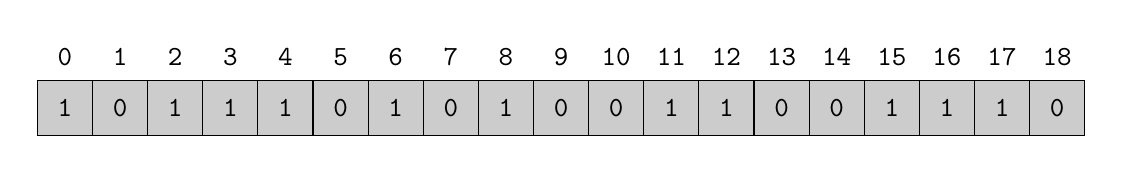
\begin{tikzpicture}[
			font=\ttfamily,
			array/.style={matrix of nodes,nodes={draw, minimum size=7mm, fill=gray!40},column sep=-\pgflinewidth, row sep=0.5mm, nodes in empty cells,
				row 1/.style={nodes={draw=none, fill=none, minimum size=5mm}},
				row 1 column 1/.style={}}]
			
			\matrix[array] (array) {
				0 & 1 & 2 & 3 & 4 & 5 & 6 & 7 & 8 & 9 & 10 & 11 & 12 & 13 & 14 & 15 & 16 & 17 & 18\\
				1 & 0 & 1 & 1 & 1 & 0 & 1 & 0 & 1 & 0 & 0 & 1 & 1 & 0 & 0 & 1 & 1 & 1 & 0\\
			};
		\end{tikzpicture}
		\centering
		\caption{Maximum-length ($18$ bits) input address acquired through \code{i\_w}.}
	\end{figure}
	
	
	
	The first two bits, $S_0$ and $S_1$, represent the output selection, which determines which output lane is chosen. There are $4$ possible output 8-bit lanes, \code{z\_0} through \code{z\_3}, so the joined bits $S_0 S_1$ uniquely identify an active output port (using a demultiplexer).
	The next zero to $16$ bits are the address. They are ordered LSB to MSB, thus they have to be stored right-to-left, and finally padded with zeros up to 16 bits if $k < 16$.
	

	\begin{figure}[htb]
		\centering
		
		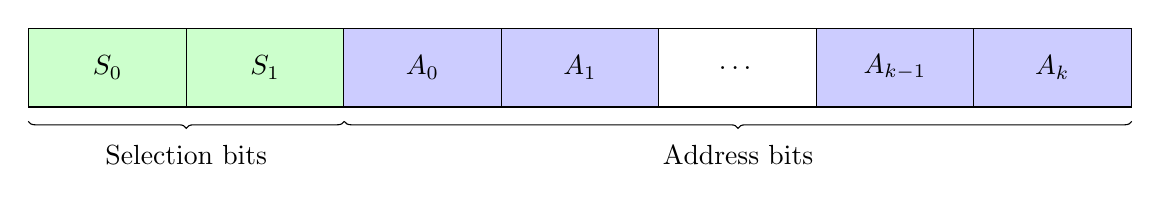
\begin{tikzpicture}
			\foreach \c/\i [count=\n] in  
			{green!20/$S_0$,green!20/$S_1$,blue!20/$A_0$,blue!20/$A_1$,white/\dots,blue!20/$A_{k-1}$,blue!20/$A_k$} 
			\node[draw,fill=\c,minimum height=1cm,minimum width = 2cm,xshift=\n*2cm](N\n){\i} ;
			
			\draw [decoration={brace,mirror,raise=5pt},decorate] (N1.south west) --  node[below=10pt]{$\mathrm{\normalsize{Selection\ bits}}$}(N2.south east); 
			\draw [decoration={brace,mirror,raise=5pt},decorate] (N2.south east) --  node[below=10pt]{$\mathrm{\normalsize{Address\ bits}}$}(N7.south east);
		\end{tikzpicture}
		\centering
		\caption{Dividing the input signal in two types, \textit{select} and \textit{address}. $k \in [0,16]$.}
	\end{figure}
	
	
	
	\subsubsection{Memory Access}
	
	The component can interface with a RAM component (\href{https://docs.xilinx.com/v/u/2017.3-English/ug901-vivado-synthesis}{Single-Port Block RAM Write-First Mode}) to do the actual fetching of the address and return an 8-bit word.
	
	The main component can interact with the memory via a set of pins:
	
	\begin{itemize}
		\item \code{o\_mem\_addr} is the memory address input, where the received address should be transmitted. It is a 16-bit port.
		\item \code{i\_mem\_data} is the return data lane from the memory, where the requested data will be received. It is an 8-bit port.
		\item \code{o\_mem\_we} and \code{o\_mem\_en} are enable bits for reading and writing operations. The write enable should always be off, the read enable should be on when actively interacting with the component.
	\end{itemize}
	
	
	\begin{figure}[H]
		\centering
		
		$\begin{NiceArray}{ll}[hvlines]
			0000000000000000 & D_0 \\
			0000000000000001 & D_1 \\
			0000000000000010 & D_2 \\
			0000000000000011 & D_3 \\
			0000000000000100 & D_4 \\
			000000000000010\ & D_5 \\
			\Cdots \\
			1111111111111101 & D_{2^{16} -3} \\
			1111111111111110 & D_{2^{16} -2} \\
			1111111111111111 & D_{2^{16} - 1} \\
		\end{NiceArray}$
		
		\caption{Memory representation. Each line represents a mapping between an address and a data word.}
	\end{figure}

	\subsubsection{Output and State Preservation}

	The component's output signals are divided as follows:
	
	\begin{itemize}
		\item \code{o\_done} is the done status bit, notifying that the component has completed its work cycle and is not active;
		\item \code{o\_z0} through \code{o\_z3} are the output ports to send the actual output signal(s) to. They are 8-bit ports, since the data contained in the RAM memory is at 8 bit. Those ports should be hooked to an internal register to allow stateful output processing.
	\end{itemize}
	
	Once the main component receives the data word from memory, the specifications impose that the following must happen:
	
	\begin{itemize}
		\item For \code{o\_done=0}, all the output ports should transmit an all-zero signal. This should be the default behaviour;
		\item For \code{o\_done=1}, which should happen for exactly one clock cycle per component operation:
		\begin{itemize}[label=$\star$]
			\item The active output port (chosen by the selection bits $S_0 S_1$) must output the data word $D_i$ extracted from memory. The word must match the address that has been given as input during the input acquisition state;
			\item All the remaining ports should retain their previous output state. \textit{By default}, all exits start out at null, but if an output port has already been used  (read as: selected with $S_0 S_1$, set as active and had a data word $D_j$ output through it) in the past, then it should remember the last value it has used as output and retain it for the clock cycle when \code{i\_done=1}.
		\end{itemize}
	\end{itemize}

        Thus, the component must keep an internal state of the last exit data word to actually produce that output once an operation is completed.
        Also, at most one register's content is overridden with a single operation. The component does not allow for multiple (batched) operations.\\When the component is brought in the reset state (via enabling \code{i\_rst}, all the state information is lost (or rather, set to zero, like at the beginning).



	\newpage

	\section{Architecture}

	The design for the described component fits very well for a finite state machine pattern. We described the model using a fsm and implemented that in VHDL.

        Note that a single-fsm design has been chosen as the current solution for its increased simplicity and consistency (for the problem at hand), when compared to multi-fsm VHDL components.



	\begin{figure}[H]
		\centering
		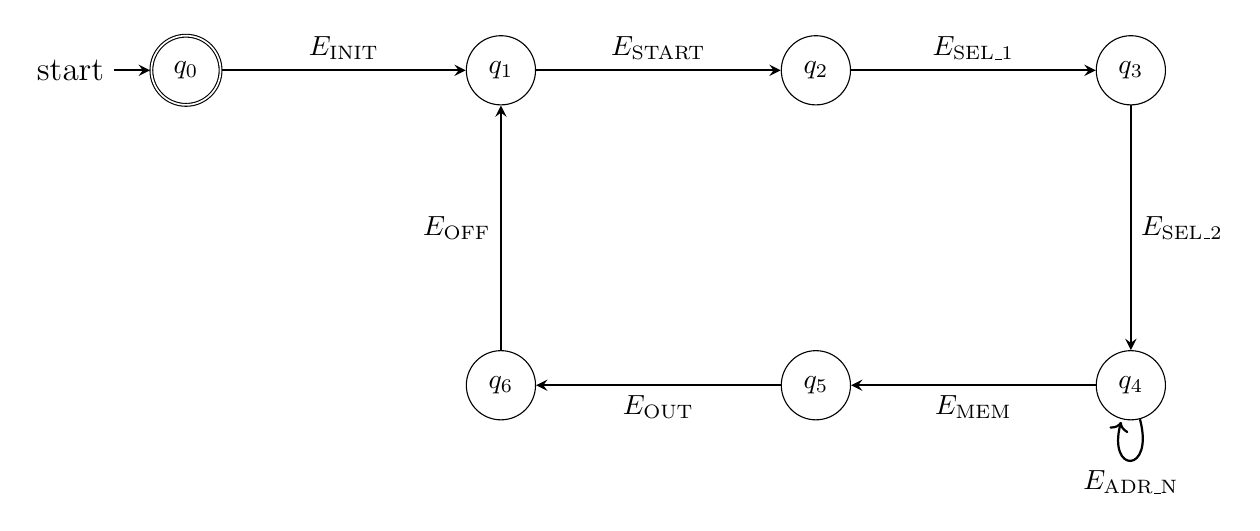
\begin{tikzpicture} [node distance = 4cm,
			on grid,
			auto,
			every state/.style = {draw = black},
			every initial by arrow/.style = {font = \large,
				text = black,
				thick,-stealth
			}
			]
			% States
			\node (q0) [state, initial, accepting, initial text = {start}] {$q_0$};
			\node (q1) [state, right = of q0] {
				$q_1$ \nodepart{lower} $\mathrm{idle}$
			};
			\node (q2) [state, right = of q1] {$q_2$};
			\node (q3) [state, right = of q2] {$q_3$};
			\node (q4) [state, below = of q3] {$q_4$};
			\node (q5) [state, left = of q4] {$q_5$};
			\node (q6) [state, left = of q5] {$q_6$};
			%Transitions
			\path [-stealth, thick, text = black]
			
			(q0) edge node  {$E_\mathrm{INIT}$} (q1)
			(q1) edge node  {$E_\mathrm{START}$} (q2)
			
			(q2) edge  node  {$E_\mathrm{SEL\_1}$} (q3)
			(q3) edge node {$E_\mathrm{SEL\_2}$} (q4)
			
			(q4) edge [loop below]  node {$E_\mathrm{ADR\_N}$} ()
			
			
			(q4) edge node {$E_\mathrm{MEM}$} (q5)
			(q5) edge node {$E_\mathrm{OUT}$} (q6)
			(q6) edge node {$E_\mathrm{OFF}$} (q1);
			%(q2) edge [bend left] node [below] {$E_{2,0}$}  (q0)
			%(q2) edge [bend left] node [below left] {$E_{2,1}$} (q1);
		\end{tikzpicture}
	\end{figure}


	The machine has n states, each one with its specific purpose, and each state transition is marked by an event.
	
	The states are cyclic, meaning that one component operation is translated into a full cycle of the normal states.

		
		
		
	\subsection{Reset State ($q_0$)}
	
	This is the fsm's initial state, and it allows for proper component initialization and output setting.
        This state is supposed to initialize all the internal signals and register contents. Once that is done, the machine automatically transitions to the $q_1$ (Idle) state
	
	This state is reached when the component is first turned on (it is hardcoded in the component's logic), and every time the \code{i\_rst} signal is asserted on a rising clock edge.
	
	
	
	\subsection{Idle State ($q_1$)}
	
	The idling state is used when there is no ongoing operation, and the \code{i\_start} signal has not been asserted yet. This state just waits for the start signal to be asserted, and switches to the $q_2$ state. The state is indeed labeled throughout the code as \code{WAIT\_START}, since its sole purpose is to detect a rising edge on the start signal. Once that happens, the fsm transitions to $q_2$
	
	

	\subsection{Selection Bits Acquisition State ($q_2$ and $q_3$)}

	Those two states are used for reading the first and second output selection bits, $S_0$ and $S_1$, which are stored in appropriate signals for output selection later on.
	
	We are guaranteed to have \code{i\_start} asserted for at least two clock cycles by the project specifications, letting us ignore the case where the signals falls before.
	
	
	\subsection{Address Bits Acquisition State ($q_4$)}
	
	This state is used to acquire a variable number (from 0 to 16) of address bits, until the \code{i\_start} signal goes low. The first address bit is $b_0$ (the 0-th bit, with address value $2^0$). Each new bit is stored as the next significant bit. The $i$-th bit has a relative address-value of $2^i$.
	
	This state can be repeated for up to 16 times.

        Once the start signal goes low, we move to the $q_5$ state.
	
	\subsection{Memory Access State ($q_5$ and $q_5'$)}

        This state is actually two, sequentially executed states.
	The received address is sent out to the memory. Its read bit is enabled. 
        Then in the next state we wait for the return data to be transmitted by the RAM component, and once we receive them we can go ahead to $q_6$.

	\subsection{Output State ($q_6$)}
	
	The received data word is written in the expected exit's register (through a demux), the \code{o\_done} bit is set, and then all the registers will output their content on \code{0\_z0} through \code{o\_z3}.

	The done bit will be reset to zero on the next clock cycle, and the state will become idle again.


 \vspace{1cm}
	

        \begin{figure}[H]
	       \centering
	       \lstinputlisting[style=demostyle]{state.vhdl}
	       \caption{The component's VHDL status enumeration}
        \end{figure}




\newpage

    \section{Results}
        \subsection{Synthetized Component}

        The component can be logically divided in the fllowing blocks:

	\begin{itemize}
			\item A fsm module handling input acquisition, RAM interaction and clock/reset logic;
			\item An output module with a demultiplexer and registers for holding information.
	\end{itemize}

        \begin{figure}[H]
        	\centering
        	\includegraphics[width=0.7\linewidth]{schema}
        	\caption{The component's simplified schematics}
        	\label{fig:schema}
        \end{figure}



        \subsection{Output Logic}
 
	For the testing phase of the project, it was chosen to implement the following three main features:

	\begin{itemize}
			\item \code{o\_done} is the done status bit, notifying that the component has compleated its work cycle;
			\item \code{o\_z0} through \code{o\_z3} are the output ports to send the actual output signal(s) to. 8-bit ports.
	\end{itemize}

        \newpage

            \subsubsection{Reset Signal}

            An important constraint imposed by the specifics is the reset signal, which bring the fsm to the initial state independently from the current state. 
            

            \begin{figure}[H]
            	\centering
            	\includegraphics[width=0.7\linewidth]{RST_TB.png}
            	\caption{The fsm signal being reset to default after the reset signal has been asserted}
            	\label{fig:schema}
            \end{figure}




            \subsubsection{Done Signal}

            The done signal is used to communicate that a result has been produced.
            The output signals will be activated and produce their data, and after one clock cycle everything goes back to zero.


            \begin{figure}[H]
            	\centering
            	\includegraphics[width=0.7\linewidth]{O_DONE_SETTING.png}
            	\caption{All the output signals going back to an 8 bit zero exit value after the done bit becomes low}
            	\label{fig:schema}
            \end{figure}


	
	   \subsection{Post-Synthesis Analysis}
        The designed component is successfully synthesizable and produces the following utilization report. No latches are generated.
        

        \vspace{1cm}
            \begin{figure}[H]
            	\centering
            	\includegraphics[width=0.7\linewidth]{report.png}
            	\caption{Component usage table, from TLC's \code{report\_utilization} command in Vivado}
            	\label{fig:schema}
            \end{figure}

            

        \newpage
	\section{Conclusions}

        The designed component meets the project's specifics and has been tested with the provided test benches, along with some external tests as well to ensure it works under all conditions.

        We analyzed our solution and a single circuit operation takes between 5 and 21 clock cycles.        

        An interesting aspect for the current circuit is that it is mostly stateless. Apart from holding the memory words which have been previously extracted and output through a designated exit bus, the entire component functionality and logic is completely stateless. It relies on the external memory component for data fetching and on the input ports for address 

        We mentioned that the component's core logic resembles an address dereferencer, given that it takes an address and gives out (mostly) a data word. This kind of circuit would model a \textit{load} assembly instruction, given that it takes a memory address and puts in a register the corresponding word

        An important note is that the component makes a few assumptions about the environment around it to work correctly, and it not resilient to changes

        The list of assumptions 

	\begin{itemize}
			\item The start signal is kept active long enough for the fsm to read the first two selection bits, and it is stopped after the maximum address size is reached:
   
                \begin{itemize}[label=$\star$]
			         \item If the \code{i\_start} signal were to be interrupted before the 2 clock cycle necessary to acquire the selection bits and address, zeros are used instead;
			         \item If the \code{i\_start} signal were to be kept high after 18 clock cycles, the incoming bit would become the MSB and shift right, removing the previous LSB.
		    \end{itemize}
      
			\item The memory takes exactly 1 clock cycle to lookup the data and return it on the \code{i\_mem\_data} port.
	\end{itemize}

        We have also explored different solutions for this specific project: specifically one which involved splitting the combinatory and synchronous logic in two different VHDL processes to decouple the state changes and the circuit logic in different units, but we preferred to stick with a single process given the project specifications did not require that kind of approach.


\end{document}


